\documentclass[conference]{IEEEtran}
\IEEEoverridecommandlockouts
% The preceding line is only needed to identify funding in the first footnote. If that is unneeded, please comment it out.
\usepackage{cite}
\usepackage{amsmath,amssymb,amsfonts}
\usepackage{algorithmic}
\usepackage{graphicx}
\usepackage{textcomp}
\usepackage{xcolor}
\usepackage{hyperref}
\def\BibTeX{{\rm B\kern-.05em{\sc i\kern-.025em b}\kern-.08em
    T\kern-.1667em\lower.7ex\hbox{E}\kern-.125emX}}

\hyphenation{Q6.16}
\hyphenation{Q12.18}

    
\begin{document}

\title{FPGA Fractal Ray Marcher}
%{\footnotesize \textsuperscript{*}Note: Sub-titles are not captured in Xplore and
%should not be used}
%\thanks{Identify applicable funding agency here. If none, delete this.}
%}

\author{\IEEEauthorblockN{Thanadol Chomphoochan}
\IEEEauthorblockA{\textit{Department of Electrical Engineering and Computer Science} \\
\textit{Massachusetts Institute of Technology}\\
Cambridge, Massachusetts \\
tcpc@mit.edu}
\and
\IEEEauthorblockN{Dillon DuPont}
\IEEEauthorblockA{\textit{Department of Electrical Engineering and Computer Science} \\
\textit{Massachusetts Institute of Technology}\\
Cambridge, Massachusetts \\
ddupont@mit.edu}}

\maketitle

\begin{abstract}
We present a design for a hardware-based graphics pipeline that uses the ray marcher algorithm to render infinitely large scenes on an FPGA. Our design utilizes approximately 0.2 MB of Block RAM on a Nexys4 DDR Artix-7 FPGA board to render a 400 by 300 grayscale image at a rate of 30-60 frames per second. We implement, test, and evaluate the performance of our design, and discuss potential improvements.
\end{abstract}

\begin{IEEEkeywords}
Digital systems, Field programmable gate arrays, Computer graphics
\end{IEEEkeywords}

% ------------------------------------------------

\section{Top Level Organization}

Our pipeline has five main components: user control, ray marcher, BRAM manager, VGA control, and Ethernet subsystem. The user control interprets user inputs and informs the ray marcher of the scene to be rendered. The ray marcher, the main component of our project, has a finite state machine that dispatches rendering jobs to internal "Ray Units." These units compute the color at a requested pixel with variable latency, and the ray marcher controller FSM forwards the results to the frame buffer. The BRAM manager manages input/output routing to two frame buffers of equal size. The ray marcher writes to one buffer and the VGA control reads from the other, ensuring that each frame is displayed without artifacts. Finally, the Ethernet subsystem allows the user to export the currently rendered image via Ethernet. See Fig.~\ref{block-diagram} for the block diagram.


\begin{figure*}
\centerline{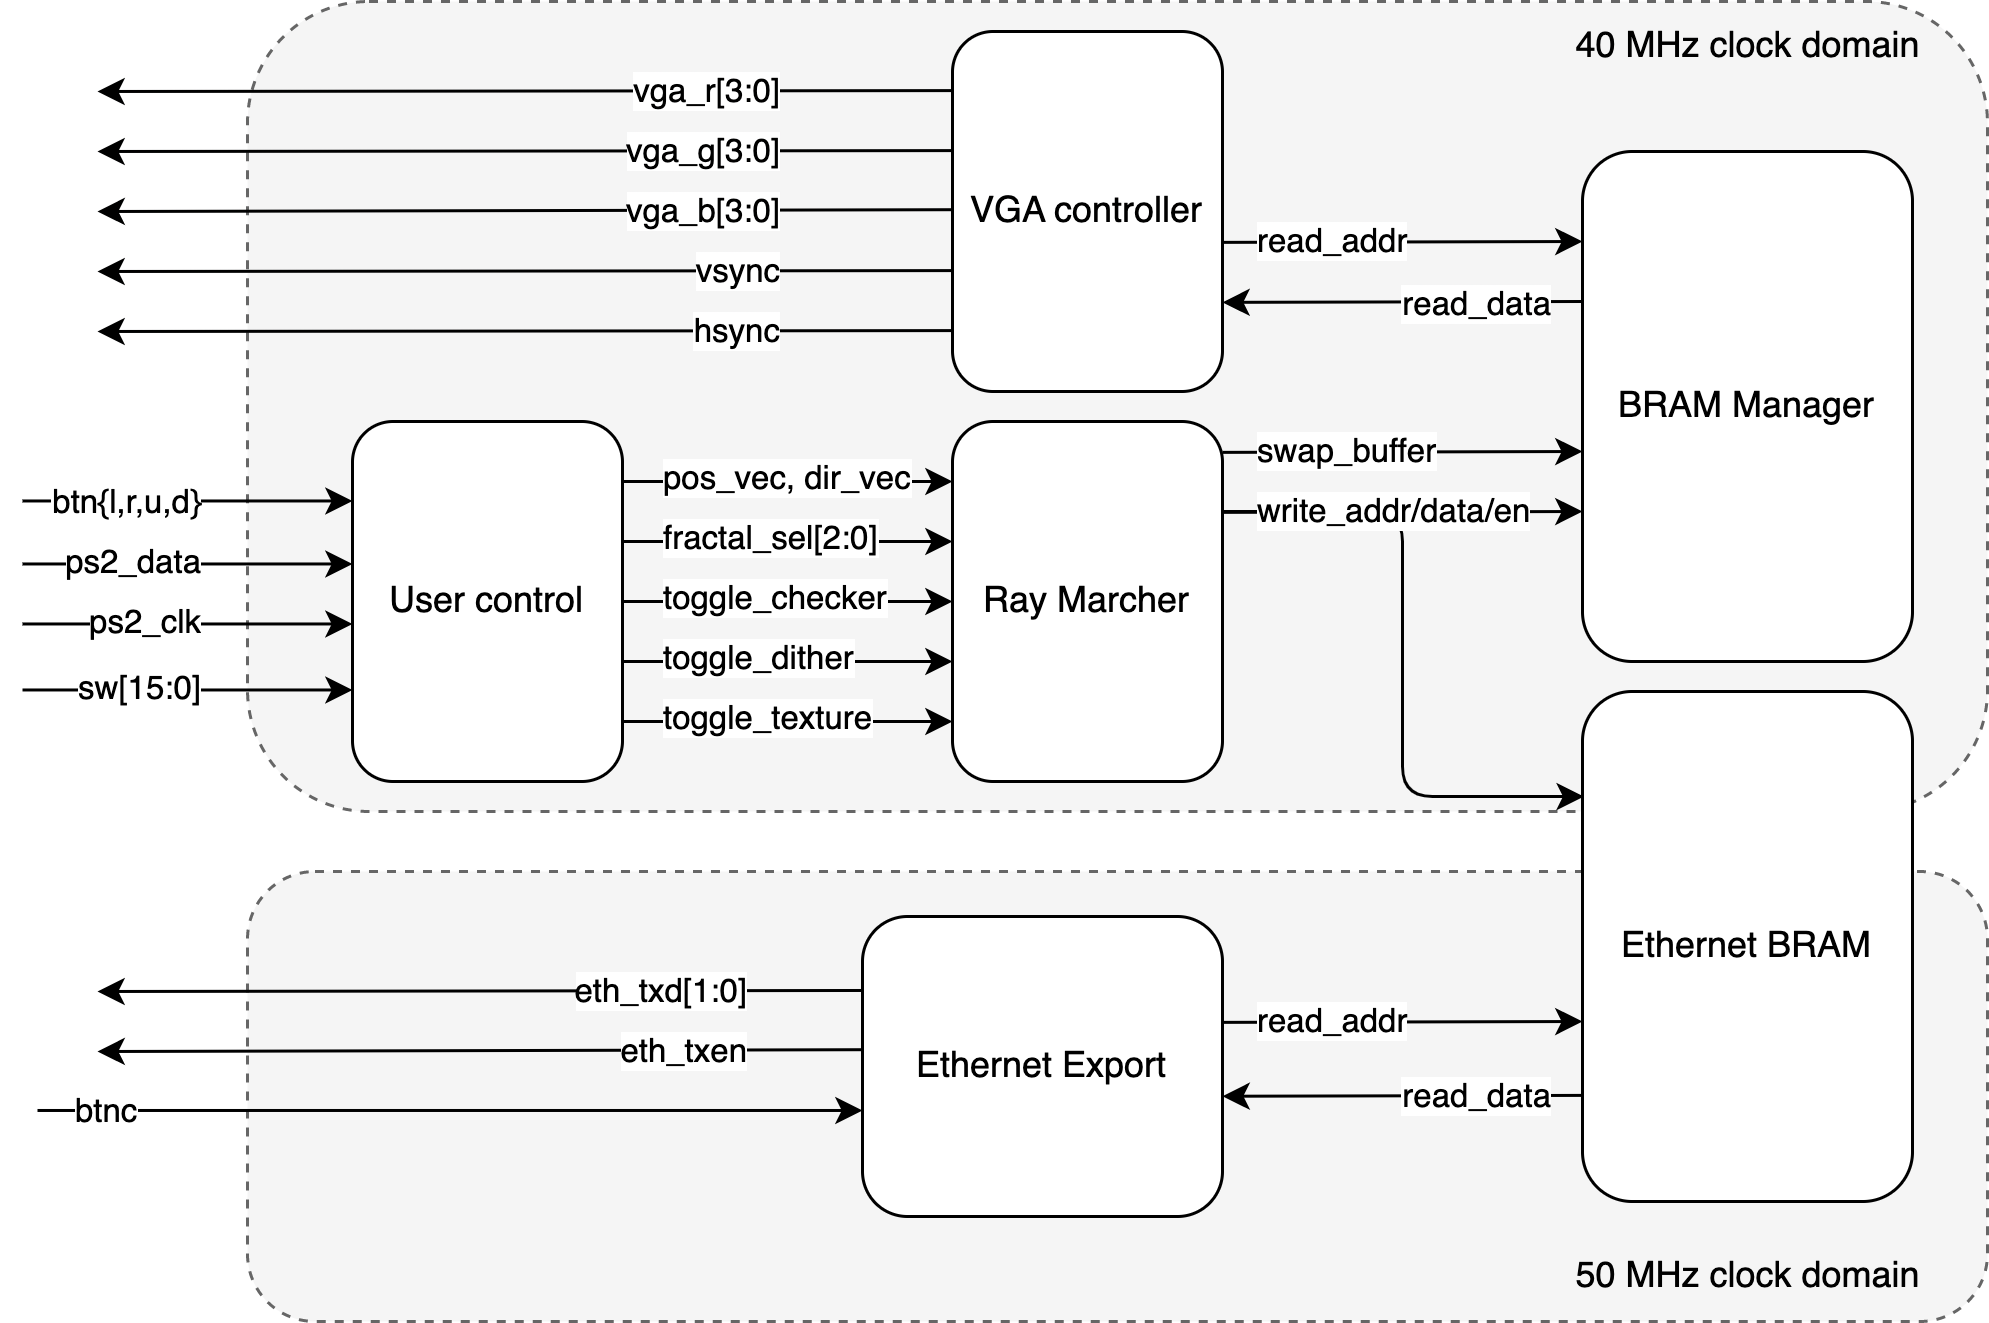
\includegraphics[width=0.8\textwidth]{top_block_diagram.png}}
\caption{Block diagram for the top level of the system}
\label{block-diagram}
\end{figure*}

All modules outside of the Ethernet subsystem run on a 40 MHz clock, consistent with the requirements for outputting an 800 by 600 image at 60 Hz via VGA. The Ethernet subsystem runs on a 50 MHz clock.

Source code listing for the project can be found at \texttt{\href{https://tcpc.me/fpga-ray-marcher}{https://tcpc.me/fpga-ray-marcher}}.

% ------------------------------------------------

\section{Number Representation}


Given the nature of this project, we require a compact but precise enough representation of real numbers that enable efficient synthesis for basic arithmetic operations such as adding and multiplying.

We use the Q6.16 fixed-point representation to represent real numbers, where the first 6 bits denote the whole part of the number (including the sign bit) and the last 16 bits represent the fractional part. This allows us to represent numbers in the range $[-2^5, 2^5)$ with precision up to $2^{-16}$. This representation is sufficiently large and precise enough for the purposes of this report. A 3D vector can then be easily represented as three Q6.16 fixed-point numbers.


Operations can be easily implemented and used in SystemVerilog thanks to type definitions and automatic functions. Addition, subtraction, negation, and comparison work in the same way as integers. Multiplication also works similarly but requires shifting the result right by 16 bits to get the correct magnitude. We do not implement division, but we do implement the inverse square root function for vector normalization. This is accomplished by shifting the input to the range $[0.5, 1]$, estimating the answer by linearly interpolating between $1/\sqrt{0.5}$ and $1/\sqrt{1}$, performing two iterations of Newton's method, and shifting the output to the correct magnitude. Note that we only handled inputs of at least 0.5 because our system never has to find the inverse square root of a smaller number. Two iterations of Newton's method are enough to get a result as precise as our number representation can handle (See Fig.~\ref{newton-graph}). The inverse square root function is implemented as a folded circuit to reduce the critical path length and DSP utilization.

\begin{figure}
\centerline{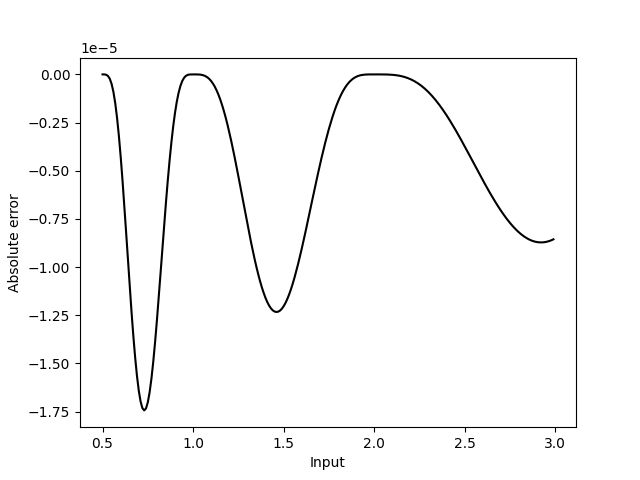
\includegraphics[scale=0.5]{newton.png}}
\caption{Absolute error for the inverse square root function}
\label{newton-graph}
\end{figure}

To use the fixed-point arithmetic and vector arithmetic library, we included \texttt{src/fixed\_point\_arith.svh} and \texttt{src/vector\_arith.svh} at the beginning of each file. We have also created test benches that automatically verify the correctness of the library. The test benches can be run through these scripts:
\begin{itemize}
    \item \texttt{test-fixed-point.sh}
    \item \texttt{test-vector.sh}
    \item \texttt{test-fp-inv-sqrt-folded.sh}
\end{itemize}


%-------------------------------------------------

\section{User Control and Keyboard Inputs}

The User Control FSM keeps track of the position and the direction of the camera in the scene. It interprets FPGA button inputs and keyboard inputs and moves the camera accordingly. The User Control also allows the user to change the fractal being rendered, changes the movement speed, and toggles various rendering features such as color display, dithering, and checkerboard rendering, via the switches on the FPGA board.

There are two movement modes for the user: Walking and Translation. In walking mode, the user can move the camera forward or backward and turn left or right. In translation mode, the user can move the camera up, down, left, or right, relative to the plane of the current camera.

Keyboard inputs are interpreted using a combination of the PS/2 Decoder implemented in Lab 2 from the first half of 6.205 in Fall 2022 and our own (relatively trivial) finite state machine for keeping track of relevant buttons' states. The user can walk using the WASD buttons and translate using the arrow keys without selecting a movement mode.

The User Control FSM also features collision detection. Keyboard input is used to calculate the next position. The next position is then fed into an SDF Query submodule (to be explained), which returns the distance from the next position to the nearest wall. This allows the User Control FSM to easily check if the player is trying to move into a wall, as the FSM will only update the current position if the SDF Query is above a specific distance.

%-------------------------------------------------

\section{Ray Marcher Controller}

The Ray Marcher Controller dispatches Ray Units and maintains internal counters for rows, columns, and Ray Unit indices. On each clock cycle, it checks if the current Ray Unit is free. If it is, the controller copies its output to the frame buffer, assigns the pixel, and increments the column and Ray Unit counters. If the unit is busy, the controller increments the Ray Unit index and waits for the next clock cycle. For easier implementation, there is an "end of row" state to increment the row counter and reset the column counter. When all pixels have been rendered, the Ray Marcher Controller emits a "new frame" signal to the BRAM manager, which makes the current frame available to the VGA controller and allows the Ray Marcher Controller to write to the other buffer. See Fig.~\ref{ray-marcher-control} for the state diagram.

The ray marcher increments both integer and normalized coordinates (in the range $-1$ to $1$) by precomputed amounts, eliminating the need for two multiplications within the Ray Units. This also eliminates the need for large numbers, as the rendering logic does not require full integer coordinates. The ray marcher's implementation can be found in \texttt{src/ray\_marcher.sv}. Non-synthesizable instructions in this file print the rendered scene in a text format, allowing the ray marcher to be simulated entirely in software and its output viewed with a Python script. This script can be run with sim-ray-marcher.sh.

The ray marcher controller was developed independently of the Ray Units. To test its ability to correctly assign jobs and handle outputs, we implemented dummy Ray Units that stall for a random number of cycles. (See \texttt{src/ray\_unit\_dummy.sv}.) The test bench can be run with \texttt{test-ray-marcher.sh}, and outputs should be manually examined.

\begin{figure}[htbp]
\centerline{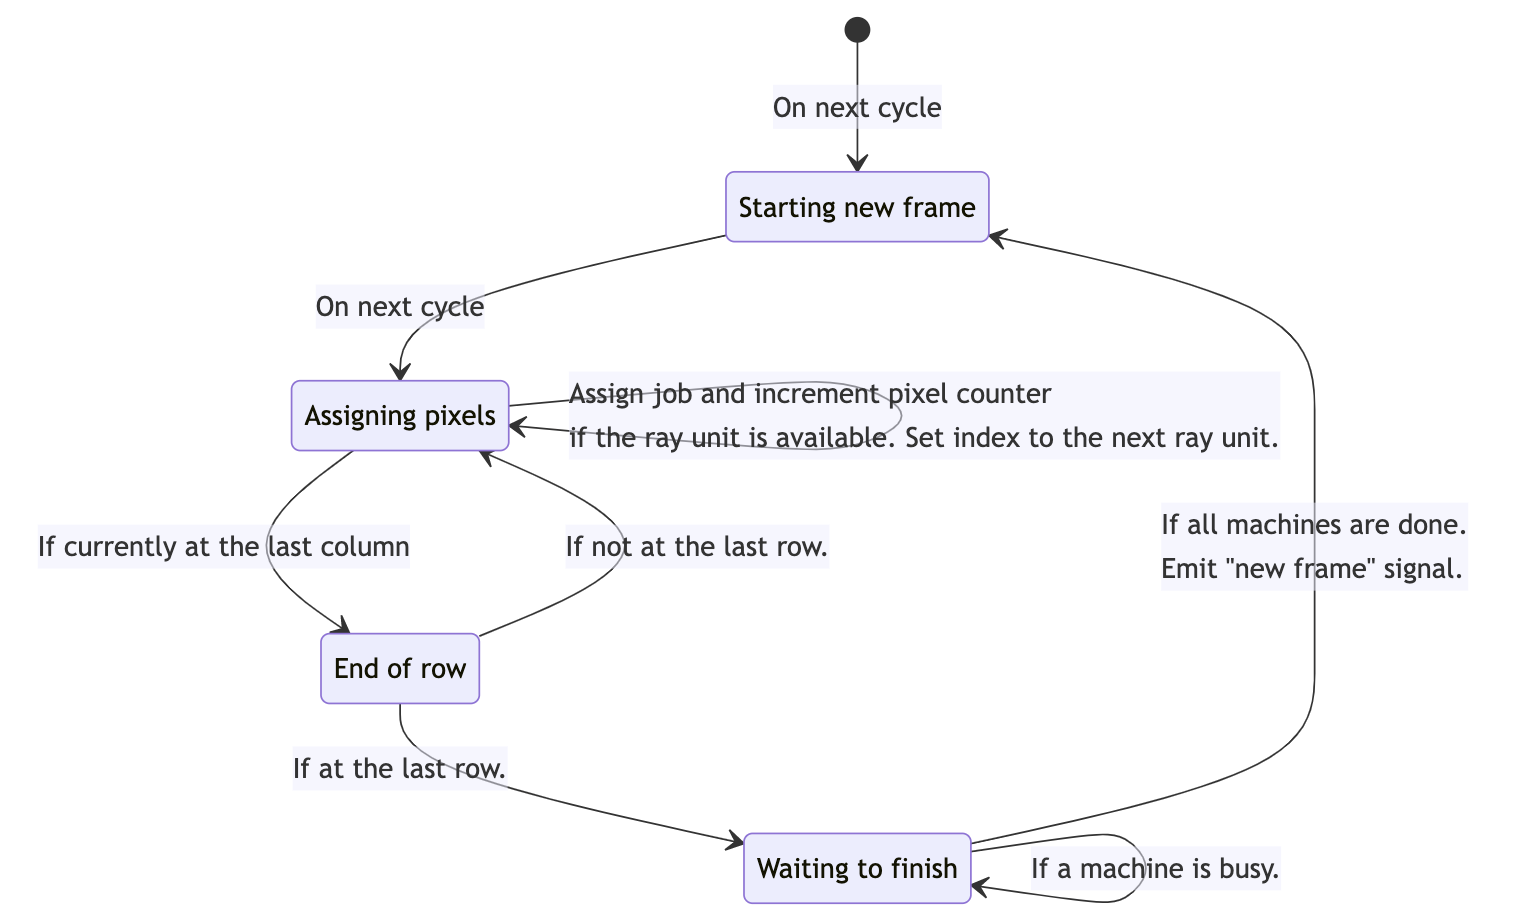
\includegraphics[scale=0.4]{ray-marcher-control.png}}
\caption{State diagram for the Ray Marcher Controller}
\label{ray-marcher-control}
\end{figure}


%-------------------------------------------------

\section{Ray Unit}

The Ray Unit takes in pixel coordinates and uses the ray marching algorithm to find the color information at the current pixels. It is implemented with multiple different submodules; the Ray Generator, the Texture Sampler, the SDF Query, and the Marcher Logic FSM. The general organization can be seen in Fig.~\ref{ray-block-diagram}.

\begin{figure*}
\centerline{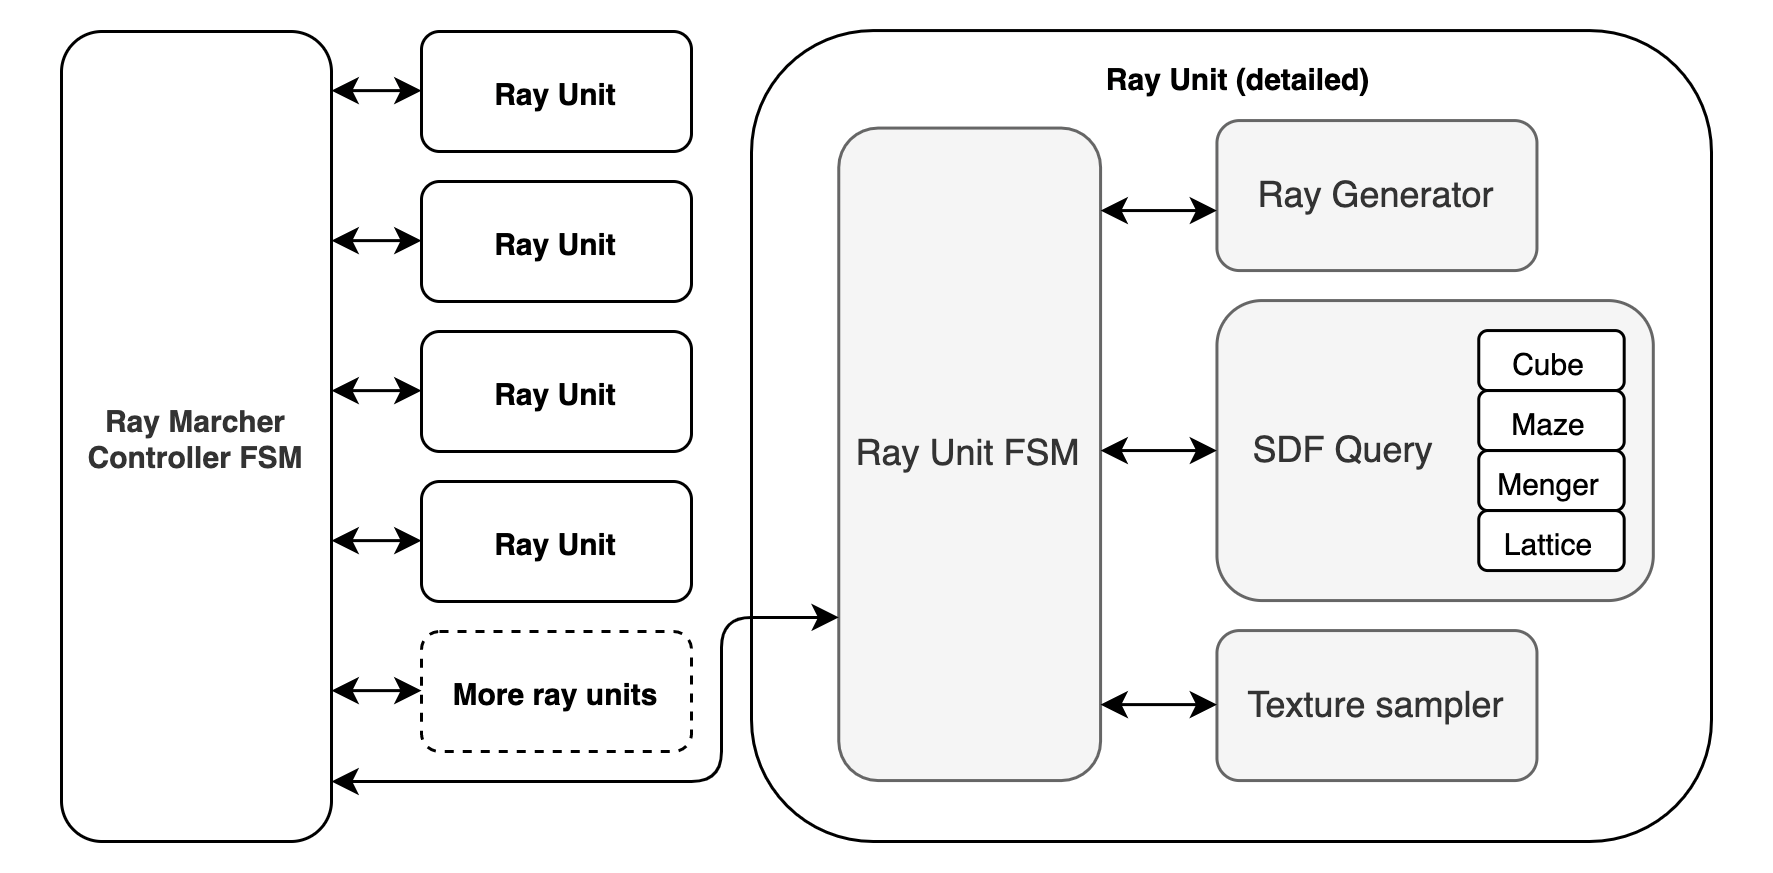
\includegraphics[width=0.8\textwidth]{ray_block_diagram.png}}
\caption{Block diagram for the Ray Marcher}
\label{ray-block-diagram}
\end{figure*}

\subsection{Ray Generator}

The Ray Generator is a module that sets up the initial state of the Marcher FSM by taking a 2D screen position and camera vectors as input and outputting a normalized 3D directional vector for each pixel. It is folded to fit more Ray Units within the FPGA's DSP blocks. The module is defined in \texttt{src/ray\_generator\_folded.sv}.


\subsection{Texture Sampler}

The Texture Sampler is a module that generates procedural textures based on input data from the Ray Unit. The primary inputs are the world position of a ray hit and the original color value of the ray. The texture is generated by dividing the world into rectangles and modulating the color at the edges of these rectangles, creating a tiling "brick wall" texture. The module is defined in \texttt{src/texture\_sampler.sv}.

\subsection{SDF Query}

The SDF Query is a module that stores scene geometry information using a Signed Distance Function (SDF). This function takes a 3D position vector as input and outputs a signed fixed-point value representing the distance between the input position and the closest surface in the scene. This allows for easy creation of scenes with fractals and infinitely detailed geometry, and the resulting depth value can be used to calculate surface normals and approximate shadows. The module is defined in \texttt{src/sdf\_query.sv}.

\begin{figure}[htbp]
\centerline{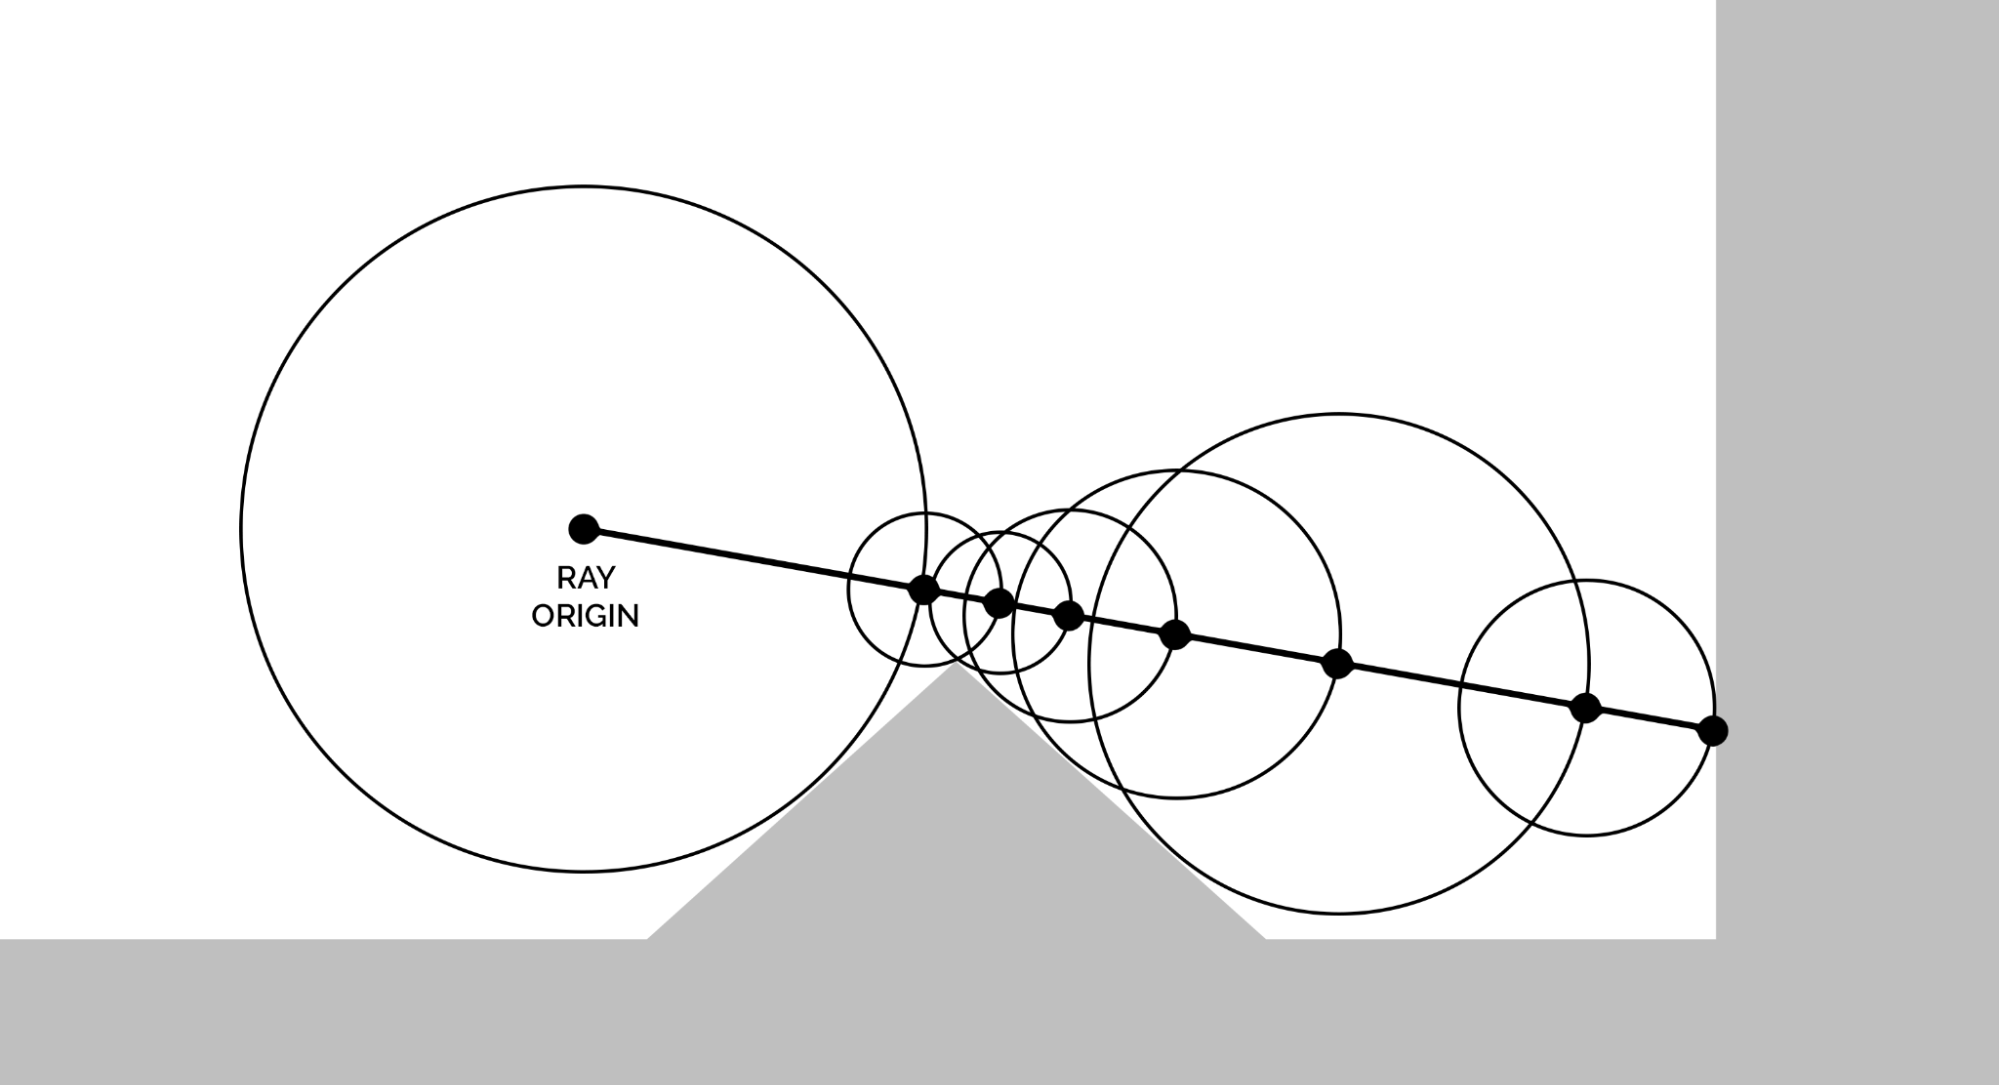
\includegraphics[scale=0.1]{ray-march-viz.png}}
\caption{Visualization of the SDF Ray Marching algorithm. (Teadrinker, CC BY-SA 4.0, via Wikimedia Commons)}
\label{ray-march-viz}
\end{figure}

\subsection{Marcher Logic FSM}

The Marcher Logic FSM is the top-level FSM in the Ray Unit that combines the output of the Ray Generator and the SDF Query to perform Ray Marching. After valid pixel information is received from the ray marcher controller, the Marcher Logic FSM relays that to the Ray Generator and stores the ray direction and ray position in a buffer. The FSM then queries the SDF with the current ray position. If the signed distance is above the minimum distance, it translates the ray position by scaling the ray direction by the signed distance and adding it to the current ray position, then returns to the query state for another iteration. If the signed distance is below the minimum distance, the FSM shades the current pixel using its state information and returns to the idle state. See Fig.~\ref{ray-unit-fsm}.

The shaded color for each 2D pixel is calculated using the depth value to get an approximation of shadow occlusion. Since the internal shaded value has a higher bit width than the color values of the frame buffer and the display, the Ray Unit performs ordered dithering using the screen coordinates to reduce quantization errors and simulate a higher color depth in the final image.

The Marcher Logic FSM implementation can be found in \texttt{src/ray\_unit.sv}. This file also contains instantiation of the Ray Generator and SDF Query submodules.

\begin{figure}[htbp]
\centerline{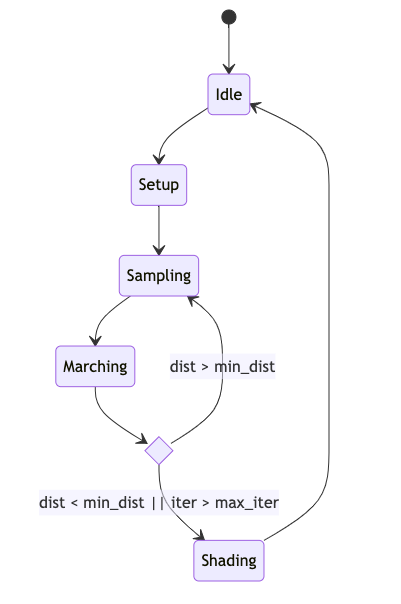
\includegraphics[scale=0.38]{ray-unit-fsm.png}}
\caption{State diagram for the Ray Unit}
\label{ray-unit-fsm}
\end{figure}

%---------------------------------------

\section{BRAM Manager and VGA Controller}

The BRAM manager owns two BRAMs, each with a depth of 400x300 and a width of 4 bits, allowing for the storage of up to two frames at the same time. The BRAM manager exposes the correct read/write ports of the BRAMs using a multiplexer. The read port corresponds to the fully rendered frame buffer and is read by the VGA controller. The write port corresponds to the frame buffer being rendered by the ray marcher. When a frame is finished, the ray marcher notifies the BRAM manager, which changes its internal state and switches the exposed buffers. The BRAM manager was tested with \texttt{test-bram-manager.sh} and outputs were manually examined.

The VGA controller is a wrapper for the VGA signal generator from Labs 3 and 4 of 6.205 in Fall 2022. It takes the pixel count and calculates the correct address to read from the frame buffer. It also translates grayscale pixels into colored pixels by multiplying the grayscale values by constants dictated by the color setting.

%---------------------------------------

\section{Ethernet Subsystem}

The Ethernet subsystem allows the user to export the currently rendered image from the Ray Marcher to their computer via Ethernet. This is implemented by creating another frame buffer that runs on two different clock domains. The Ray Marcher, which runs on a 40 MHz clock, uses one port to write the pixel values to the frame buffer. The Ethernet Export FSM, running on a 50 MHz clock, uses the other port to read the pixel values and listen for button inputs from the user. When the export button (BTNC) is pressed, the Ethernet Export FSM sends a raw Ethernet frame consisting of the Ethernet header, 50 bytes of all-1 bits, and the frame check sequence. It then sends a frame for each row in the image, starting with the row count (4 bytes) and followed by the grayscale pixel values (400 col $\times$ 4 bits/col = 200 bytes). The user can run a Python script on their computer to listen for these Ethernet frames and render them into an image file.

To simplify the process of sending Ethernet frames, we created an Ethernet Transmission submodule (defined in \texttt{src/ether\_tx.sv}), which can be used in this manner:

\begin{enumerate}
\item The upstream module (i.e. the Ethernet Export FSM) sends a trigger signal. The submodule will start sending the preamble and the Ethernet header.
\item Once the submodule is ready to send the actual payload, it sends a "data ready" signal to the upstream module.
\item The upstream module sends data (in dibits) and eventually stops by sending a "last dibit" signal.
\item The submodule handles the frame check sequence, and also ensures that it will not send another frame again until the interframe gap has passed.
\end{enumerate}

Note that the submodule receives data in Most Significant Byte, Most Significant bit (MSB/MSb) order. The submodule internally reverses the endianness and handles all pipelining complications.

%---------------------------------------

\section{Results}

Our system can display a 12-bit RGB 400x300 image of four scenes: a cube, a box lattice, a Menger sponge tunnel, and a maze. We were able to successfully synthesize the system with up to 12 Ray Units, using 35.56\% of the available BRAMs (400 $\times$ 300 $\times$ 4 bits each $\times$ 3 buffers). The limiting factor was the number of slice LUTs and registers available, as shown in Table~\ref{table-resource}. This is surprising, as we expected to run out of DSPs first due to the large number of multiplications needed to calculate the SDFs. \footnote{The preliminary report used up to 98\% of the DSPs for a Ray Marcher with 8 Ray Units because of a bug in the previous implementation, which required us to use Q12.18 number representation rather than Q6.16.}


\begin{table}[!t]
\renewcommand{\arraystretch}{1.3}
\caption{Ray Marcher Resource Utilization}
\label{table-resource}
\centering
\begin{tabular}{c||c|c|c}
\hline
\bfseries \# Ray Units & \bfseries WNS & \bfseries Slice Util\% & \bfseries DSP Util\% \\
\hline\hline
4 & 1.946 ns & 38.42\% & 35.56\% \\
8 & 1.305 ns & 64.53\% & 45.42\% \\
12 & 0.250 ns & 92.08\% & 65.42\% \\
\hline
\end{tabular}
\end{table}

Our system measures rendering speed by attaching a frame rate counter module to the Ray Marcher's \texttt{swap\_buffer} signal. The module counts the number of frames generated and finds the average value after moving around in the scene for five seconds. The frame rates are given in Table~\ref{table-speed}. Rendering speed depends on the average number of ray marching iterations per pixel (higher for more complex scenes) and the latency of the SDF Query. For example, the SDF for cube scenes requires only one clock cycle to compute while the maze requires five, resulting in an almost five-fold difference in performance.

\begin{figure}[htpb]
\centerline{\includegraphics[width=0.45\textwidth]{result1.png}}
\caption{Menger sponge tunnel rendered on screen}
\label{result1}
\end{figure}

\begin{figure}[htpb]
\centerline{\includegraphics[width=0.45\textwidth]{result2.png}}
\caption{Infinite grid of cubes rendered on screen}
\label{result2}
\end{figure}

\begin{figure}[htpb]
\centerline{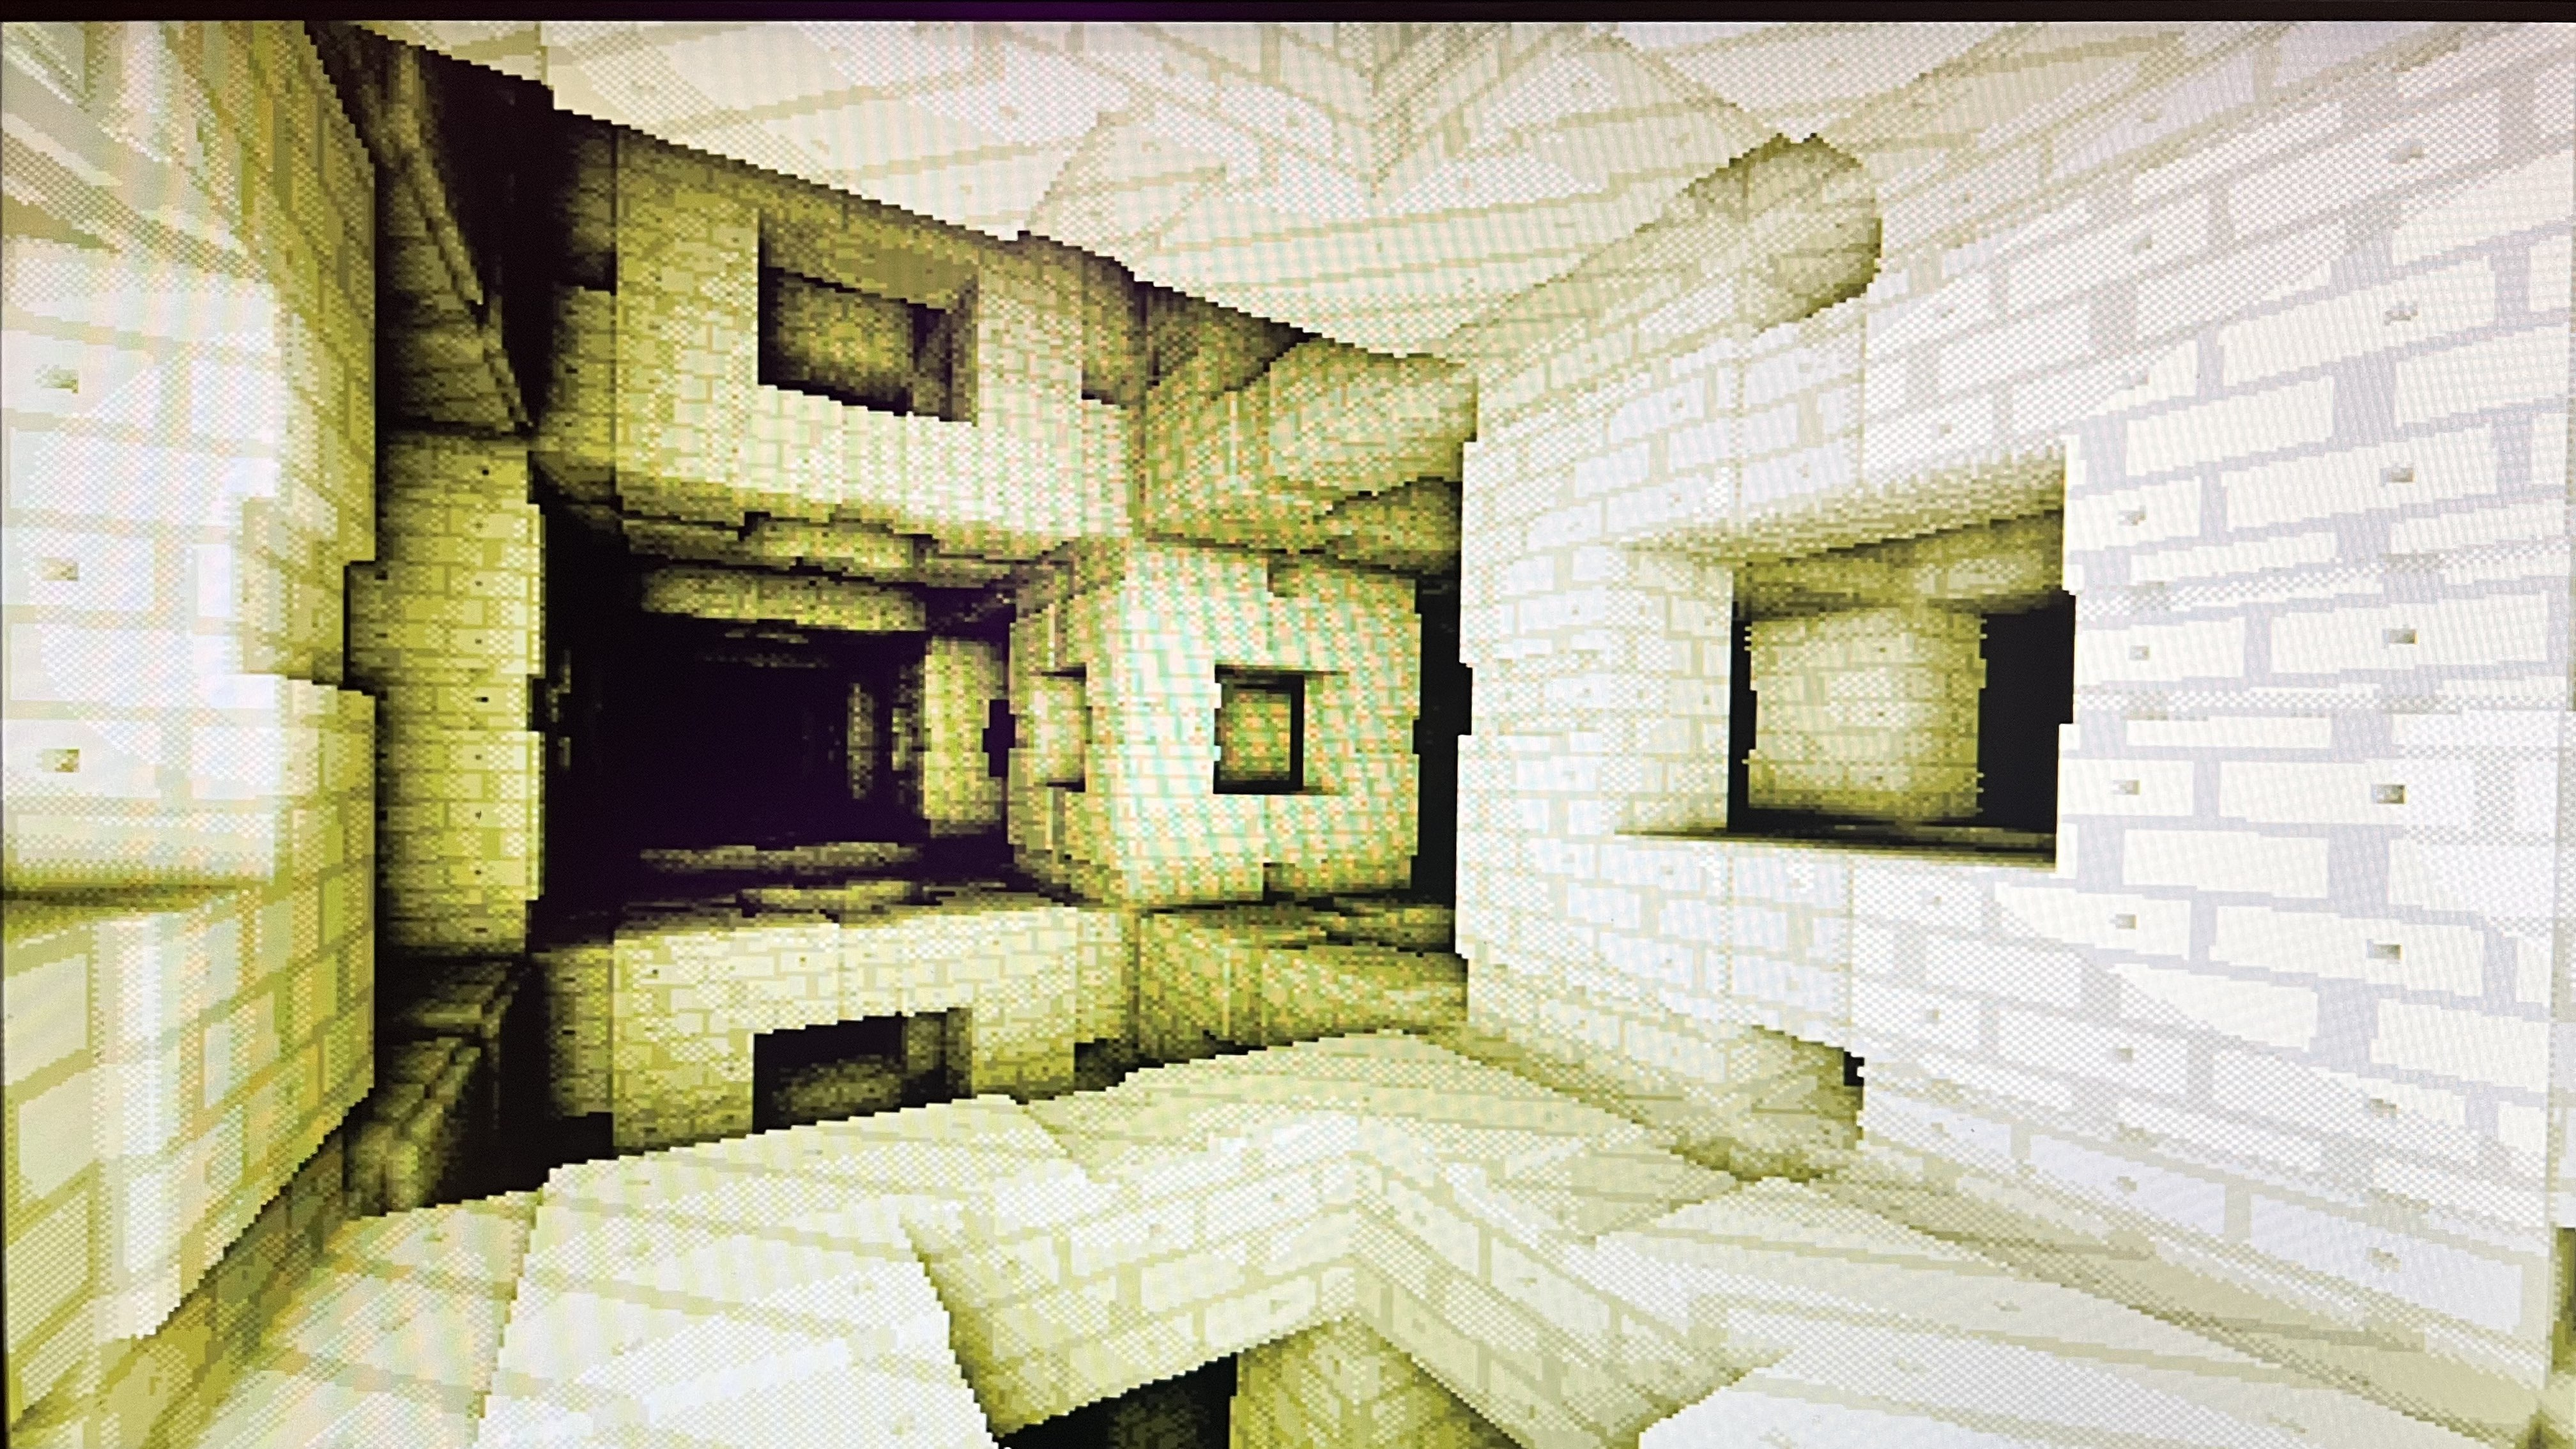
\includegraphics[width=0.45\textwidth]{result3.jpg}}
\caption{Menger sponge tunnel viewed from a different angle}
\label{result3}
\end{figure}

\begin{figure}[htpb]
\centerline{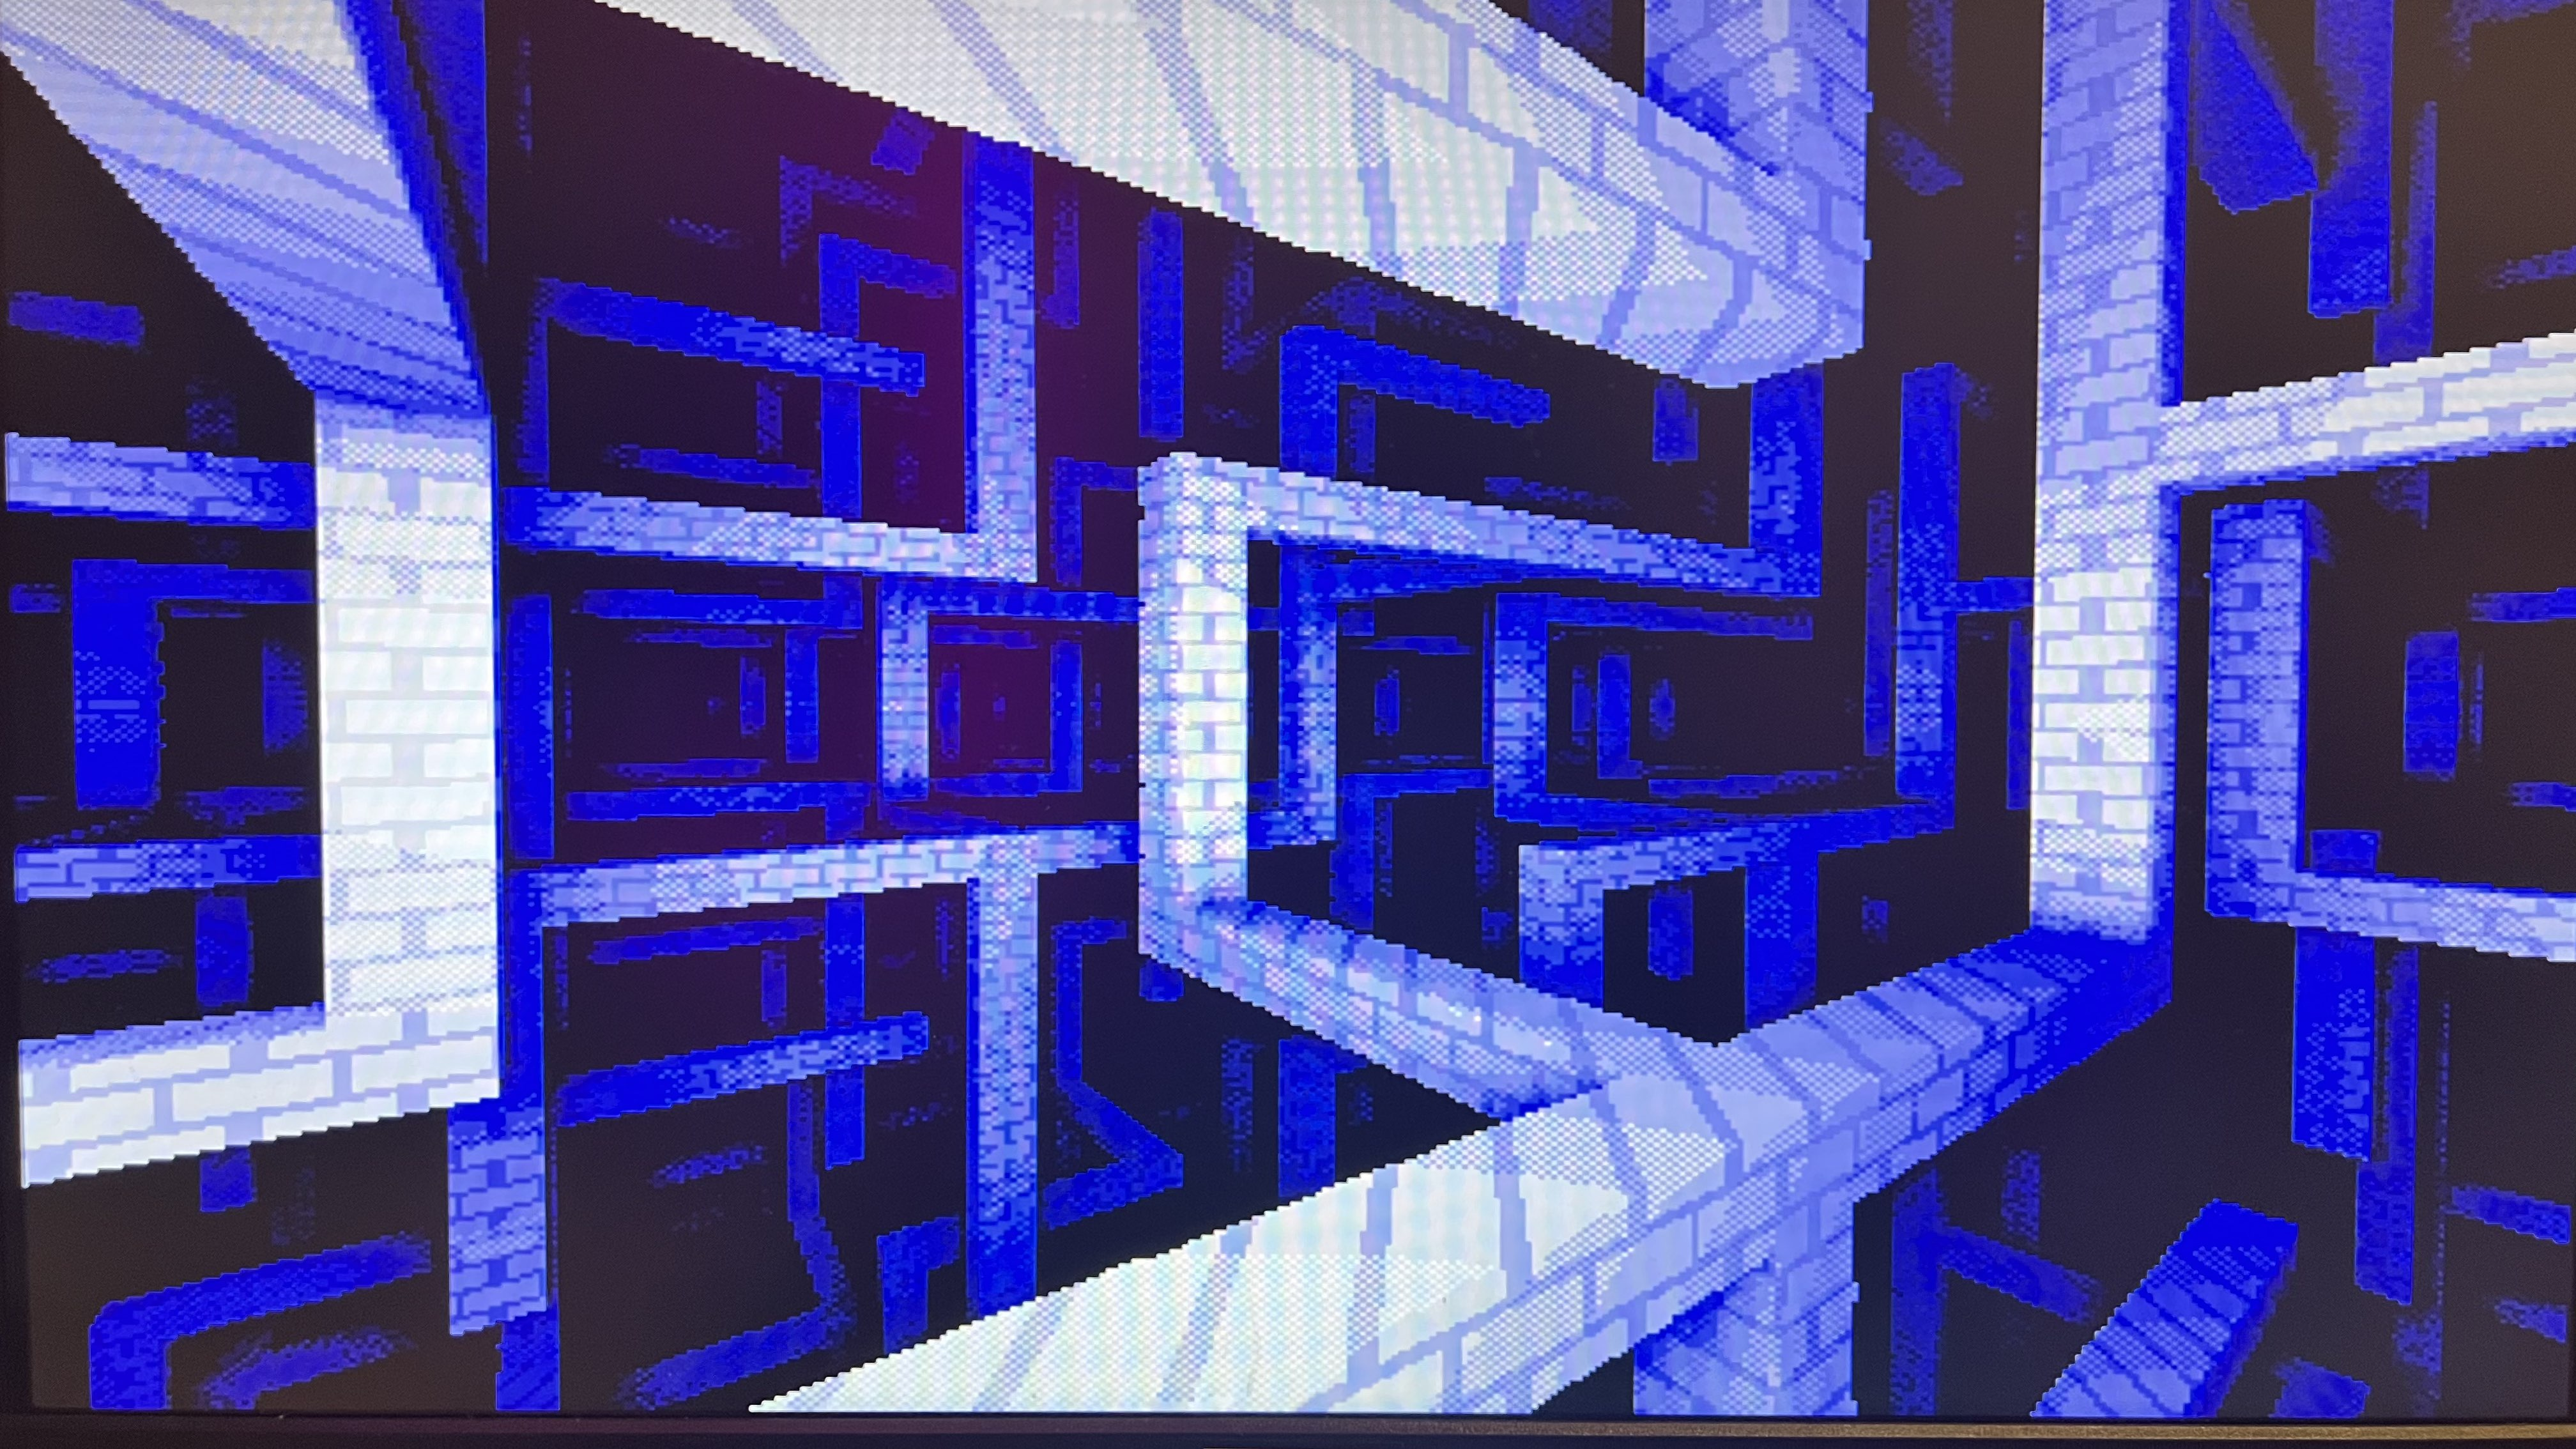
\includegraphics[width=0.45\textwidth]{result4.jpg}}
\caption{Randomized maze rendered on screen}
\label{result4}
\end{figure}


We employ a couple of rendering techniques to improve the color depth and performance. Enabling the dithering filter provides a $2 \times$ perceived color depth improvement, and checkerboard rendering, which skips every other pixel for even/odd frames, provides a $2 \times$ FPS improvement.

\begin{table}[!t]
\renewcommand{\arraystretch}{1.3}
\caption{Rendering Speed for Fractals (in Frames Per Second)}
\label{table-speed}
\centering
\begin{tabular}{c||c|c|c}
\hline
\bfseries Fractal Configuration & \bfseries 4 RUs & \bfseries 8 RUs & \bfseries 12 RUs \\
\hline\hline
Simple cube & 33 & 59 & 89 \\
Simple cube (checkerboard) & 60 & 107 & 140 \\
Infinite cubes & 27 & 50 & 70 \\
Infinite cubes (checkerboard) & 51 & 114 & 112 \\
Menger Sponge &16 & 30 & 44 \\
Menger Sponge (checkerboard) & 32 & 56 & 82 \\
Maze & 9 & 17 & 26 \\
Maze (checkerboard) & 17 & 32 & 49 \\

\hline
\end{tabular}
\end{table}

Our system achieves its primary goal, which was to display at least three fractals as a 640-by-480 image at 20 frames per second. Though our system renders at 400 by 300 resolution instead, given current resource utilization, it can easily be adapted to render at 640 by 480 resolution with fewer Ray Units. \footnote{The BRAM required for the Ethernet submodule can be shrunk significantly. The Ethernet submodule could instead query for one row at a time, disrupting the VGA Controller's operation for a few frames.} 
We chose not to follow our original target because it greatly simplifies our implementation and significantly increases performance while still maintaining the spirit of the project. We also achieve our stretch goal of implementing multiple useful features, including keyboard controls and image exporting via Ethernet, as well as rendering objects with textures and dithering. We did not implement additional rendering passes or integrate SDRAM for larger resolutions because they do not improve image quality in the software prototype enough to justify the impact on performance.

To enhance the system, we can reduce LUT slice utilization by improving our complex, nested conditional implementations and potentially pipeline the circuit better to support higher clock speeds for faster frame rates. It may also be possible to enable communication between two or more FPGA boards for further parallelization.

% -----------------------------------------------------------------------

\section{Division of Labor}

Pleng and Dillon contributed roughly equally to the project. Pleng wrote the arithmetic library, the BRAM manager, the VGA controller, and the Ray Marcher Controller, along with the necessary test benches. Pleng integrated the modules and optimized them when necessary, including folding and pipelining existing modules and micro-optimizing mathematical operations. Pleng also added keyboard inputs and Ethernet exporting. Pleng created most diagrams and figures used in the report.

Dillon focused on the graphical aspects of the project. He set up the software prototype to verify implementations and wrote most of the logic within the Ray Units, including the Ray Generator and the SDF Query. This required minimizing the use of heavy mathematical operations and verifying that the SDFs produced the intended images. Dillon added all extra graphical features, such as colors, dithering, and textures, and created the user control logic, with keyboard controls added by Pleng later in the project.

\section*{Appendix: Retrospectives}

\subsection{Notes on the design}

After completing the project, we realized that the design could be simplified. For instance, we don't need to use both ports of both BRAMs at the same time, as we only write or read to each BRAM at any given clock cycle. We could just toggle the write-enable bits, freeing up another port and allowing us to put the Ray Marcher and the VGA Controller in separate clock domains. The VGA Controller would just choose which BRAM to read from, rather than relying on the BRAM manager. (We actually had to do something similar to enable the Ethernet exporting feature anyway.)

Furthermore, performance could be improved by implementing the Ray Marcher as a pipelined circuit, eliminating the need for multiple Ray Units. This would reduce the overhead due to the Ray Controller FSM. Variable latency in the Ray Unit could be handled by adding dummy cycles or stall signals. However, the additional complexity may result in high LUT and DSP utilization and may be harder to scale (e.g. if we used multiple FPGA boards).

\subsection{Reflections on writing test benches}

In this project, we strived to work as professionally as possible to produce a good final product. This includes putting careful thought into organizing our code base and writing as many automated test benches and simulations as possible. While writing test benches requires an upfront investment, the time and headaches it has saved us are worth much more. We were surprised by how quickly we were able to get the ray marcher to work on hardware once we got the simulation working.

This lesson was made extremely clear to us in one instance: We naively thought the FPS counter was a simple enough module that did not need software testing. We put it on the hardware and were perplexed as to why it did not work. After an hour or two of stubbornly trying to debug by re-reading through the code and fixing random things, we gave in and write a simulation. It brought to light a silly typo hiding in plain sight, and we fixed the bug in five seconds. We greatly appreciated the instant karma.

Another tragic incident: We thought we could easily adapt the VGA signal generator submodule from Lab 03 to support lower resolutions. We decreased the number of bits for \texttt{hcount} and \texttt{vcount} without realizing that the maximum coordinates \textit{combined with} front/back porches and sync signals could overflow. We (or rather, Pleng, specifically) spent at least six hours trying to get a single, solid color to display on the screen. Had we spent two minutes writing a very simple simulator for the module as a sanity check, we would not have had to try to debug the more complicated modules like the Ray Marcher, when those are, in fact, not the culprit.

\subsection{Reflections on time management}

We were lucky that we were sensible enough to follow the long-revered advice of starting things early. By having a clear timeline and committing to it, we were able to build a fully functioning system by Thanksgiving break. This was really helpful at the end of the semester. We were less stressed about balancing all our obligations, knowing that we made good progress on the project and had a reasonably bounded amount of work left to finish up.


\section*{Acknowledgments}

We thank the 6.205 staff for developing this amazing class and giving us the tools necessary to succeed in the project. We are particularly grateful to Joe Steinmeyer, the course instructor, and project mentor, for helping us determine the direction of the project. We also thank Fischer Moseley and Jay Lang for being extremely amazing, cool, and helpful TAs.

\end{document}
